% generated by doc/figures.py -- edit the script, not this file
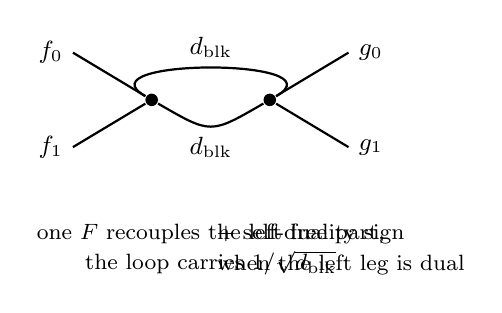
\begin{tikzpicture}[thick, every node/.style={font=\small}]
  % a closed loop carrying the shared block, with one associator on its left
  \node[circle, fill, inner sep=1.6pt] (p) at (0,0) {};
  \node[circle, fill, inner sep=1.6pt] (q) at (1.5,0) {};
  \draw (p) to[out=150,in=30,looseness=1.5] node[above] {$d_{\mathrm{blk}}$} (q);
  \draw (q) to[out=-150,in=-30,looseness=1.5] node[below] {$d_{\mathrm{blk}}$} (p);
  \draw (p) -- (-1.0,0.6) node[left] {$f_0$};
  \draw (p) -- (-1.0,-0.6) node[left] {$f_1$};
  \draw (q) -- (2.5,0.6) node[right] {$g_0$};
  \draw (q) -- (2.5,-0.6) node[right] {$g_1$};
  \node[align=center] at (0.75,-1.9)
    {\footnotesize one $F$ recouples the left free part,\\
     \footnotesize the loop carries $1/\sqrt{d_{\mathrm{blk}}}$};
  \node[align=left] at (2.4,-1.9)
    {\footnotesize $+$ self-duality sign\\ \footnotesize when the left leg is dual};
\end{tikzpicture}
